\documentclass[11pt]{article}
\usepackage[margin=1in, headheight=14pt]{geometry}
\usepackage{amsmath, amssymb}
\usepackage{hyperref}
\usepackage{enumitem}
\usepackage{algorithm}
\usepackage{algpseudocode}
\usepackage{fancyhdr}
\usepackage{tcolorbox}
\usepackage{microtype}
\usepackage{tikz}
\usepackage{pgfplots}
\pgfplotsset{compat=1.18}
\usetikzlibrary{arrows.meta, positioning, calc, shapes.geometric}

\input{notation.tex}
\input{zk-notation.tex}
\input{environments.tex}
\input{lecture-macros.tex}

\pagestyle{fancy}
\fancyhf{}
\lhead{EECS 498/CSE 598: Zero-Knowledge Proofs}
\rhead{Winter 2026}
\lfoot{Lecture 20: Incrementally Verifiable Computation and Folding}
\rfoot{\thepage}
\renewcommand{\headrulewidth}{0.4pt}
\renewcommand{\footrulewidth}{0.4pt}

% Lecture-specific macros
\tcbuselibrary{skins, breakable}

\colorlet{slidein}{red!75!black}
\colorlet{slideout}{blue!70!black}
\colorlet{slidechal}{orange!85!black}
\colorlet{slideaux}{violet!70!black}

\newcommand{\IVC}{\ensuremath{\mathsf{IVC}}}
\newcommand{\Nova}{\ensuremath{\mathsf{Nova}}}
\newcommand{\Halo}{\ensuremath{\mathsf{Halo}}}
\newcommand{\Fold}{\ensuremath{\mathsf{Fold}}}
\newcommand{\PCD}{\ensuremath{\mathsf{PCD}}}

\begin{document}

%----------------------------------------------------------------------
% Title Block
%----------------------------------------------------------------------
\begin{center}
  {\LARGE \textbf{EECS 498 / CSE 598: Zero-Knowledge Proofs}}\\[6pt]
  {\large Winter 2026}\\[4pt]
  {\large \textbf{Lecture 20: Incrementally Verifiable Computation and Folding}}\\[4pt]
  {\large Instructor: Paul Grubbs \quad
    \href{mailto:paulgrub@umich.edu}{\texttt{paulgrub@umich.edu}} \quad
    Beyster 4709}
\end{center}

\vspace{0.5em}
\hrule
\vspace{1em}

%----------------------------------------------------------------------
% Agenda
%----------------------------------------------------------------------
\section*{Agenda}
\begin{itemize}
  \item Motivating incremental proofs
  \item Incrementally verifiable computation via recursion
  \item Folding schemes and the \Nova\ viewpoint
  \item Folding relaxed $\algo{R1CS}$ instances
  \item Additive commitments and succinct folding
  \item Proof-carrying data and related extensions
\end{itemize}

\hrule
\vspace{1em}

%----------------------------------------------------------------------
\section{Motivating Incremental Proofs}
%----------------------------------------------------------------------

Consider an iterated computation defined by a transition function
\[
  z_{i+1} = F(z_i; w_i)
  \qquad\text{for } i=0,\ldots,n-1,
\]
where $z_0$ is the initial state, $z_n$ is the final state, and $w_i$ is the
step witness for the $i$-th transition.  CPU-model frontends, virtual-machine
execution, and blockchain state updates all fit this template.

Equivalently, the proving goal is to certify that repeated application of $F$
takes the initial state to the final state:
\[
  F^{(n)}(z_0)=z_n.
\]

The most direct proof strategy is to unroll all $n$ steps into one monolithic
constraint system and prove the conjunction of all transition relations at
once.  The resulting statement is
\[
  \exists\, w_0,\ldots,w_{n-1}\ \text{such that}\ 
  F(z_i; w_i)=z_{i+1}\ \text{for all } i=0,\ldots,n-1.
\]

\begin{remark}
This monolithic formulation is logically adequate, but it forces the proof
system to commit to the full execution length before proving begins.
\end{remark}

An incremental proof system is meant to preserve the same final claim while
improving the proof workflow.  Four requirements are central:
\begin{enumerate}
  \item The number of steps should not need to be fixed far in advance.
  \item The prover should avoid materializing the entire execution trace at
        once.
  \item The proof describing $i$ steps and the proof describing $i+1$ steps
        should have the same asymptotic size.
  \item Verifier work should depend only weakly on the length of the
        computation.
\end{enumerate}

Three drawbacks of the monolithic approach are especially important.
\begin{enumerate}
  \item The circuit depends on the chosen step bound $n$.
  \item Prover memory is proportional to the full unrolled computation rather
        than to a small local state.
  \item Depending on the backend, verifier preprocessing or verification time
        can also scale with $n$.
\end{enumerate}

For a step relation of size $|F|$, the slide deck emphasizes the cost profile
\[
  O(n \cdot |F|)
\]
for prover memory and verifier preprocessing in the naive unrolled approach.

%----------------------------------------------------------------------
\section{Incrementally Verifiable Computation via Recursion}
%----------------------------------------------------------------------

\begin{definition}[Incrementally verifiable computation]
An incrementally verifiable computation scheme maintains a proof object
$\Pi_i$ for each prefix of an iterated computation such that $\Pi_i$ certifies
the correctness of the first $i$ applications of $F$, and $\Pi_i$ can be
updated to $\Pi_{i+1}$ with asymptotically unchanged proof size.
\end{definition}

\subsection{Recursive Verification}

Valiant's recursive approach augments the step relation into a larger
computation $F'$ that performs two tasks:
\begin{enumerate}
  \item verify a proof $\pi_i$ asserting that $(F')^i(z_0)=z_i$;
  \item check one further transition from $z_i$ to $z_{i+1}$.
\end{enumerate}

The output of the augmented computation is a new proof $\pi_{i+1}$ asserting
that
\[
  (F')^{i+1}(z_0)=z_{i+1}.
\]
At the base case, a distinguished default proof symbol $\bot$ is used in place
of a prior recursive proof.

\begin{center}
\resizebox{0.96\textwidth}{!}{%
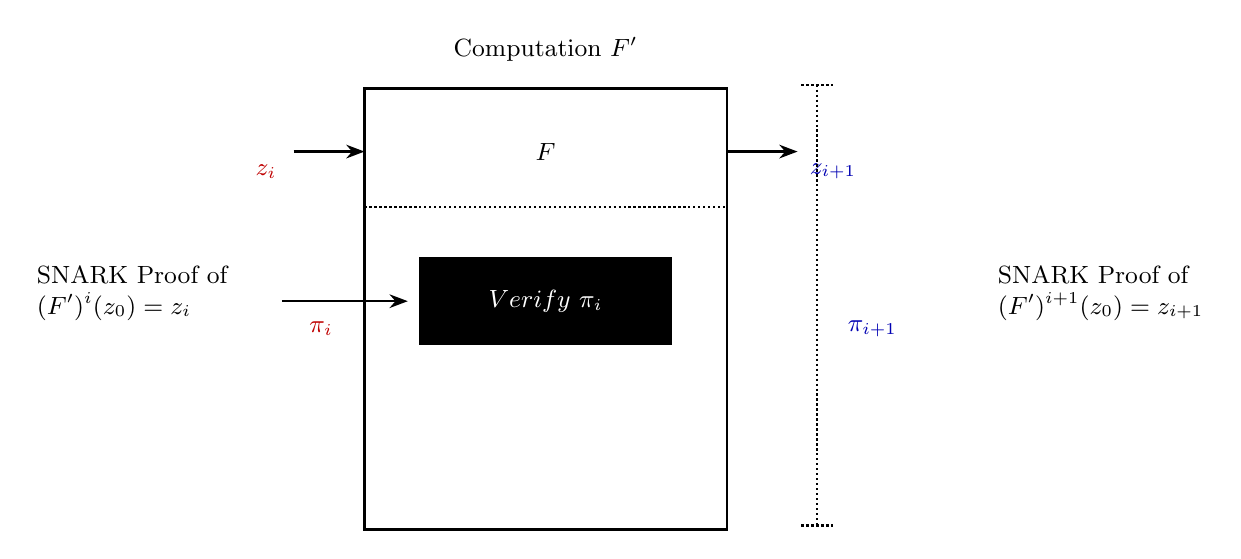
\begin{tikzpicture}[every node/.style={font=\small}]
  \draw[thick] (0,0) rectangle (4.6,5.6);
  \draw[densely dotted, thick] (0,4.1) -- (4.6,4.1);
  \node at (2.3,6.1) {Computation $F'$};
  \node at (2.3,4.8) {$F$};
  \node[draw, fill=black, text=white, minimum width=3.2cm, minimum height=1.1cm] at (2.3,2.9) {$\algo{Verify}\ \pi_i$};

  \draw[-Stealth, thick] (-0.9,4.8) -- (0,4.8);
  \node[text=slidein] at (-1.25,4.55) {$z_i$};
  \draw[-Stealth, thick] (4.6,4.8) -- (5.5,4.8);
  \node[text=slideout] at (5.95,4.55) {$z_{i+1}$};

  \node[align=left] at (-2.95,3.0) {SNARK Proof of\\$(F')^i(z_0)=z_i$};
  \draw[-Stealth, thick] (-1.05,2.9) -- (0.55,2.9);
  \node[text=slidein] at (-0.55,2.55) {$\pi_i$};

  \draw[densely dotted, thick] (5.75,5.65) -- (5.75,0.05);
  \draw[densely dotted, thick] (5.55,5.65) -- (5.95,5.65);
  \draw[densely dotted, thick] (5.55,0.05) -- (5.95,0.05);
  \node[text=slideout] at (6.45,2.55) {$\pi_{i+1}$};
  \node[align=left] at (9.35,3.0) {SNARK Proof of\\$(F')^{i+1}(z_0)=z_{i+1}$};
\end{tikzpicture}%
}

\smallskip
\emph{Valiant-style recursive update: the augmented computation $F'$ verifies
the prior proof and advances the next transition.}
\end{center}

\begin{proposition}
If the recursive verifier embedded in $F'$ is sound and each step transition is
checked correctly, then $\pi_n$ certifies the correctness of the entire
sequence
\[
  z_0 \to z_1 \to \cdots \to z_n.
\]
\end{proposition}

\begin{proof}[Proof sketch]
Each proof $\pi_{i+1}$ certifies one valid transition together with the
validity of $\pi_i$.  Induction on $i$ propagates correctness back to the base
case.  The final proof $\pi_n$ therefore compresses the correctness of the
entire chain of recursive updates.
\end{proof}

\begin{remark}
Recursive verification shifts the proof burden into the verifier circuit of the
next step.  Trusted-setup recursive SNARKs therefore rely on specialized curve
cycles whose base and scalar fields match across the recursion, for example
cycles with
\[
  \#E_1(\F_p)=q
  \qquad\text{and}\qquad
  \#E_2(\F_q)=p.
\]
Transparent recursive systems avoid that setup, but inherit a larger
in-circuit verifier.
\end{remark}

\subsection{Deferred Verification}

\Halo\ refines the recursive-verification paradigm by partially checking the
incoming proof $\pi_i$ and deferring the remaining work into an accumulator
$\mathsf{acc}_i$.  The augmented computation carries forward both the next state
and the next accumulator.

\begin{center}
\resizebox{0.96\textwidth}{!}{%
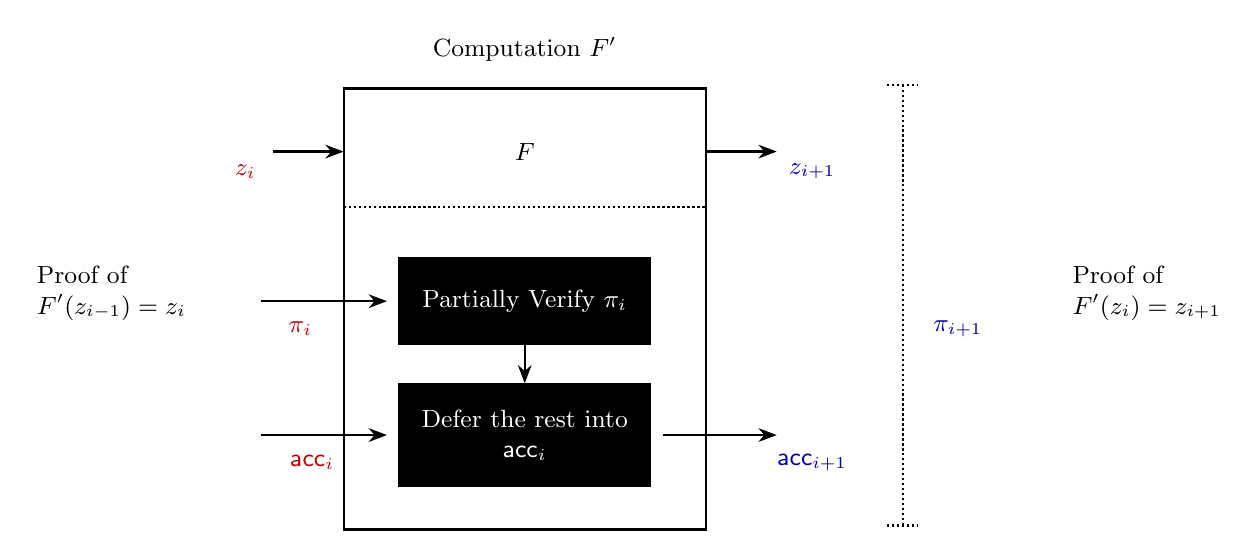
\begin{tikzpicture}[every node/.style={font=\small}]
  \draw[thick] (0,0) rectangle (4.6,5.6);
  \draw[densely dotted, thick] (0,4.1) -- (4.6,4.1);
  \node at (2.3,6.1) {Computation $F'$};
  \node at (2.3,4.8) {$F$};
  \node[draw, fill=black, text=white, minimum width=3.2cm, minimum height=1.1cm] (pv) at (2.3,2.9) {Partially Verify $\pi_i$};
  \node[draw, fill=black, text=white, minimum width=3.2cm, minimum height=1.3cm, align=center] (acc) at (2.3,1.2) {Defer the rest into\\$\mathsf{acc}_i$};
  \draw[-Stealth, thick] (pv.south) -- (acc.north);

  \draw[-Stealth, thick] (-0.9,4.8) -- (0,4.8);
  \node[text=slidein] at (-1.25,4.55) {$z_i$};
  \draw[-Stealth, thick] (4.6,4.8) -- (5.5,4.8);
  \node[text=slideout] at (5.95,4.55) {$z_{i+1}$};

  \node[align=left] at (-2.95,3.0) {Proof of\\$F'(z_{i-1})=z_i$};
  \draw[-Stealth, thick] (-1.05,2.9) -- (0.55,2.9);
  \node[text=slidein] at (-0.55,2.55) {$\pi_i$};
  \draw[-Stealth, thick] (-1.05,1.2) -- (0.55,1.2);
  \node[text=slidein] at (-0.4,0.85) {$\mathsf{acc}_i$};
  \draw[-Stealth, thick] (4.05,1.2) -- (5.5,1.2);
  \node[text=slideout] at (5.95,0.85) {$\mathsf{acc}_{i+1}$};

  \draw[densely dotted, thick] (7.1,5.65) -- (7.1,0.05);
  \draw[densely dotted, thick] (6.9,5.65) -- (7.3,5.65);
  \draw[densely dotted, thick] (6.9,0.05) -- (7.3,0.05);
  \node[text=slideout] at (7.8,2.55) {$\pi_{i+1}$};
  \node[align=left] at (10.2,3.0) {Proof of\\$F'(z_i)=z_{i+1}$};
\end{tikzpicture}%
}

\smallskip
\emph{\Halo\ carries forward an accumulator that records the deferred part of
the previous proof verification.}
\end{center}

The structural change is important: the recursive circuit no longer fully
replays the prior verifier.  Nevertheless, partial verification remains
expensive, and generating the recursive proof $\pi_i$ is still concretely and
asymptotically costly.

%----------------------------------------------------------------------
\section{Folding Schemes and the \Nova\ Viewpoint}
%----------------------------------------------------------------------

\subsection{Claims Rather Than Proofs}

The central idea behind \Nova\ is to reduce claims rather than to verify proofs
inside the recursive computation.  Two claims are maintained at step $i$:
\begin{itemize}
  \item a local claim $u_i$ describing the most recent transition
        $F'(z_{i-1}) = z_i$;
  \item an accumulated claim $U_i$ summarizing all earlier iterations,
        namely the claim that $(F')^{i-1}(z_0)=z_{i-1}$.
\end{itemize}

A folding procedure maps the pair $(u_i, U_i)$ to a new accumulated claim
$U_{i+1}$ of the same asymptotic size.  The recursive computation only needs to
check that the fold was performed correctly.

\begin{definition}[Folding scheme]
Let $\calR$ be a relation.  A folding scheme for $\calR$ is an interactive
protocol that takes two claims $(u_1,w_1),(u_2,w_2) \in \calR$ and produces a
folded claim $(u,w)$ satisfying the following properties:
\begin{enumerate}
  \item \textbf{Completeness.} If the input claims are satisfiable, then the
        folded claim is satisfiable.
  \item \textbf{Knowledge soundness.} Producing a valid folded witness implies
        knowledge of valid witnesses for the input claims.
  \item \textbf{Succinctness.} Folding is asymptotically cheaper than checking
        an instance from scratch.
\end{enumerate}
\end{definition}

\subsection{Public-Coin and Non-Interactive Folding}

When the folding protocol is public coin, Fiat--Shamir converts it into a
non-interactive folding scheme.  The output is a short transcript
\[
  \mathsf{tr}
\]
that records the prover messages together with the verifier challenge derived
from the Fiat--Shamir transform.

Given a non-interactive folding scheme for an NP relation, the augmented
computation $F'$ can check folding by running only the folding verifier on the
pair $(u_i,U_i)$ and the transcript $\mathsf{tr}$.  The witness for that step
contains two pieces of data:
\begin{enumerate}
  \item the execution trace witnessing $F(z_{i-1}) = z_i$;
  \item the folding prover state needed to produce the transcript
        $\mathsf{tr}$ and the next folded witness $W_{i+1}$.
\end{enumerate}

The recursion pattern therefore changes from ``verify a prior SNARK'' to
``verify a short folding transcript''.

\begin{remark}
Knowledge soundness alone allows the final output of the incremental proof to
be the pair $(z_n, U_n)$.  Zero knowledge and stronger compression can be added
later by wrapping the folded claim in an outer SNARK.
\end{remark}

%----------------------------------------------------------------------
\section{Folding \texorpdfstring{$\algo{R1CS}$}{R1CS} Instances}
%----------------------------------------------------------------------

\subsection{Naive Linear Folding}

The starting relation is $\algo{R1CS}$.  An instance consists of matrices
$A,B,C$ and a public input vector $x$.  A witness vector $W$ satisfies the
instance if, for
\[
  Z = (W,x,1),
\]
the equality
\[
  A Z \circ B Z = C Z
\]
holds componentwise.

A first attempt at folding is to sample a challenge $r \getsr \F$ and define
\[
  x = x_1 + r x_2,
  \qquad
  W = W_1 + r W_2,
  \qquad
  Z = Z_1 + r Z_2.
\]

If both input instances are satisfiable, then
\[
  C Z = C Z_1 + r C Z_2
      = A Z_1 \circ B Z_1 + r\, A Z_2 \circ B Z_2.
\]
The left-hand side of the $\algo{R1CS}$ relation expands differently:
\[
  A Z \circ B Z
  =
  A Z_1 \circ B Z_1
  + r \bigl(A Z_1 \circ B Z_2 + A Z_2 \circ B Z_1\bigr)
  + r^2 A Z_2 \circ B Z_2.
\]
The cross terms and the extra factor of $r^2$ show that naive linear folding
does not preserve the $\algo{R1CS}$ relation.

\subsection{Relaxed \texorpdfstring{$\algo{R1CS}$}{R1CS}}

\begin{definition}[Relaxed $\algo{R1CS}$]
A relaxed $\algo{R1CS}$ instance additionally includes a scalar $u$ and an
error vector $E$.  A witness vector $W$ satisfies the instance if, for
\[
  Z = (W,x,u),
\]
the equality
\[
  A Z \circ B Z = u \cdot C Z + E
\]
holds componentwise.
\end{definition}

The error vector absorbs the cross terms, and the scalar $u$ absorbs the extra
challenge factor created by folding.

\begin{center}
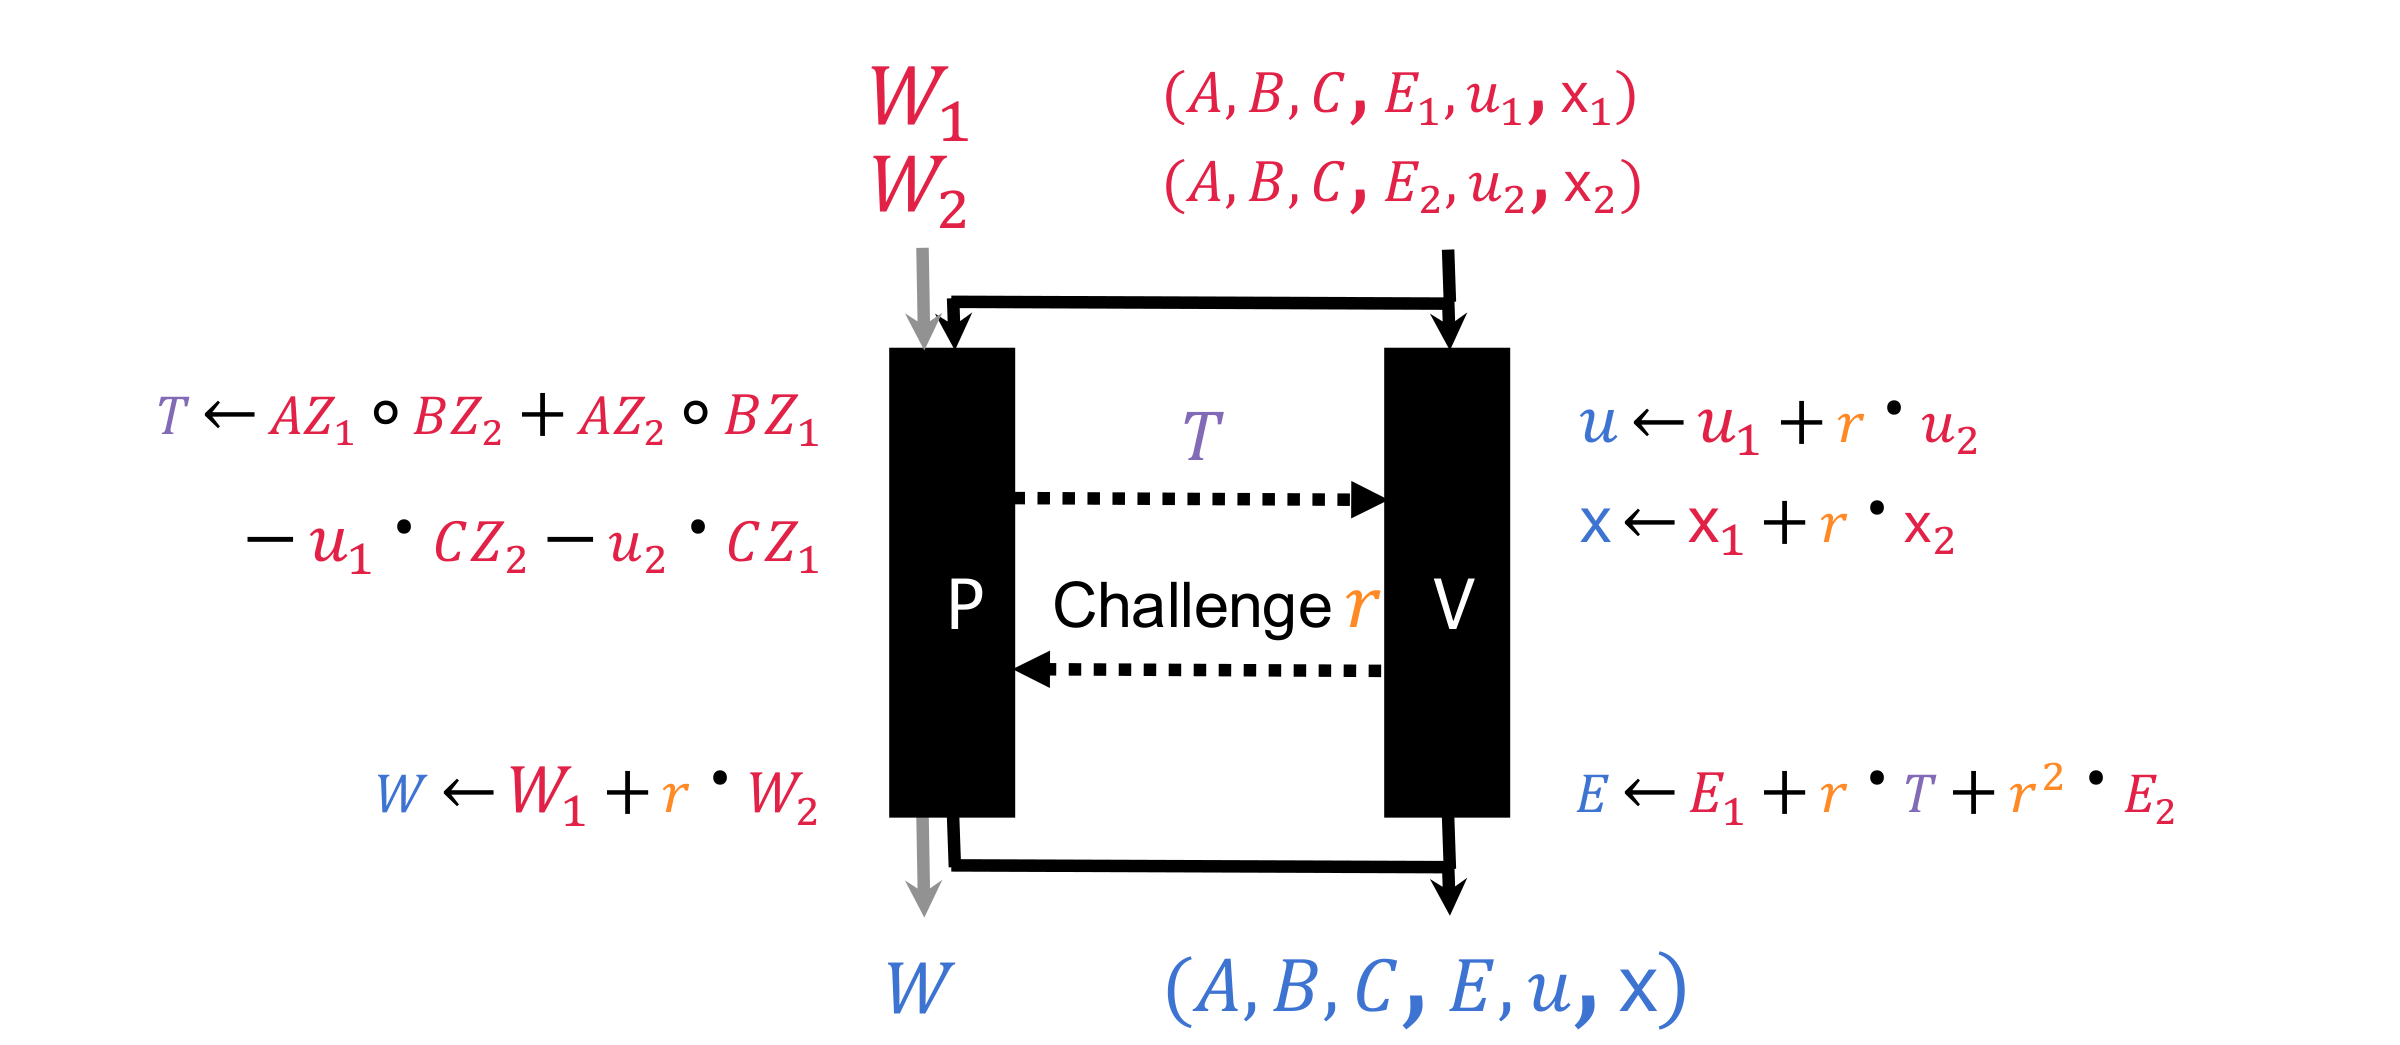
\includegraphics[width=0.94\textwidth]{figures/lecture20-relaxed-r1cs-folding.png}

\smallskip
\emph{The relaxed-$\algo{R1CS}$ folding protocol uses a cross-term vector $T$
to absorb the non-linear interaction terms created by folding.}
\end{center}

\begin{proposition}
If the two input relaxed $\algo{R1CS}$ instances are satisfiable and the cross
term vector $T$ is computed correctly, then the folded instance is also
satisfiable.
\end{proposition}

\begin{proof}[Proof sketch]
Expanding
\[
  A(Z_1+rZ_2)\circ B(Z_1+rZ_2)
\]
produces the original two satisfied relations together with the cross terms and
the $r^2$ contribution.  The update rule for $E$ is chosen exactly so that all
additional terms are absorbed into the relaxed relation.
\end{proof}

This construction is not yet succinct for two reasons:
\begin{enumerate}
  \item the verifier cannot enforce that the prover folded $W$ correctly;
  \item the error vector $E$ is as large as the witness and therefore cannot be
        handled explicitly by a succinct verifier.
\end{enumerate}

\subsection{Additive Commitments}

The remedy is to treat $(E,W)$ as witness data and include commitments to those
objects in the public statement.  The verifier sees
\[
  (A,B,C,\overline{E},\overline{W},u,x),
\]
while the prover knows openings to $\overline{E}$ and $\overline{W}$.

The committed folding protocol follows the same structure as the uncommitted
one, but the prover first sends
\[
  \overline{T} = \mathrm{com}(T)
\]
instead of sending the full cross-term vector in the clear.

\begin{center}
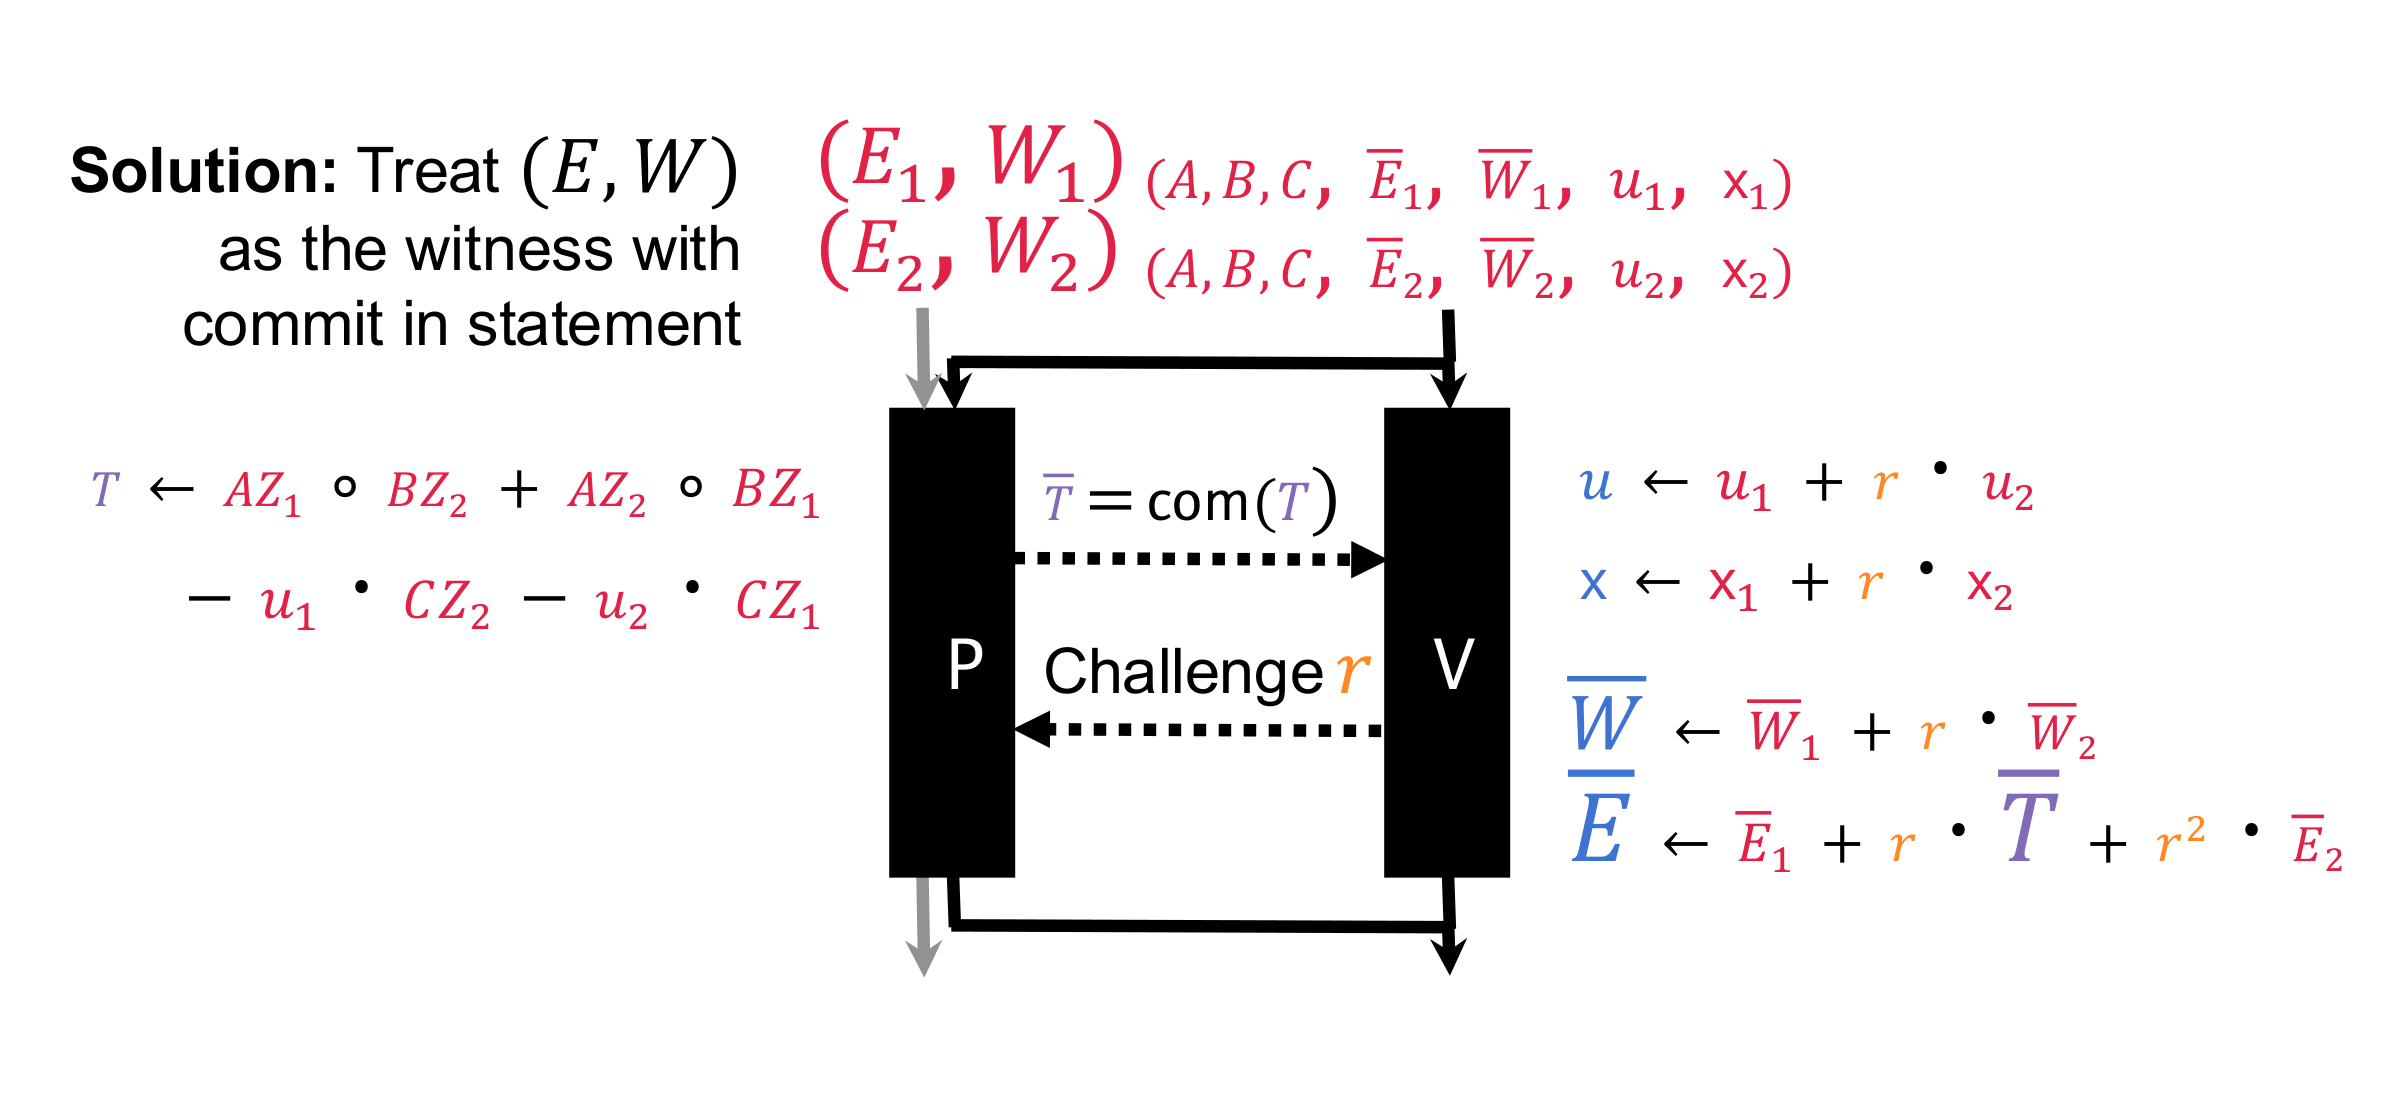
\includegraphics[width=0.94\textwidth]{figures/lecture20-additive-commitment-folding.png}

\smallskip
\emph{Additive commitments move the large witness objects $(E,W)$ into committed
form while keeping the fold transcript short.}
\end{center}

If the commitment scheme is additively homomorphic, then the verifier can fold
commitments using the same linear update rules:
\[
  \overline{W}
  \leftarrow
  \overline{W}_1 + r \overline{W}_2,
\]
\[
  \overline{E}
  \leftarrow
  \overline{E}_1 + r \overline{T} + r^2 \overline{E}_2,
\]
where $\overline{T} = \commit(T)$ is a commitment to the cross-term vector.

The prover computes the corresponding witness-side updates
\[
  W \leftarrow W_1 + r W_2,
  \qquad
  E \leftarrow E_1 + r T + r^2 E_2,
\]
while the verifier outputs only the committed instance
\[
  (A,B,C,\overline{E},\overline{W},u,x).
\]

\begin{remark}
The transcript of the fold is now short: one commitment to the cross terms, one
field challenge, and a constant number of commitment-group operations.  The
recursive verifier only needs to process this compressed transcript.
\end{remark}

%----------------------------------------------------------------------
\section{Applications and Extensions}
%----------------------------------------------------------------------

\subsection{Proof-Carrying Data}

Proof-carrying data generalizes the chain structure of $\IVC$ to a directed
acyclic graph.  Each node receives proofs from its incoming edges, checks the
local computation, and emits a proof to its outgoing edges.  Recursive
verification gives a generic construction, but folding-style reductions are
needed for practical efficiency.  At the level of abstraction, $\PCD$ is
``$\IVC$ on a DAG'' rather than on a single chain.

\begin{center}
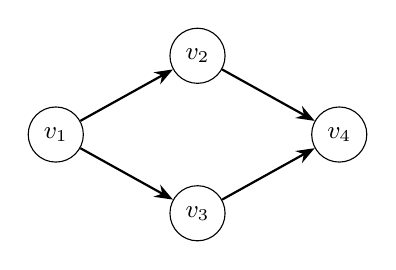
\begin{tikzpicture}[
  node/.style={draw, circle, minimum size=7mm, inner sep=0pt},
  arr/.style={-Stealth, thick},
  every node/.style={font=\small}
]
  \node[node] (a) at (0,0) {$v_1$};
  \node[node] (b) at (1.8,1.0) {$v_2$};
  \node[node] (c) at (1.8,-1.0) {$v_3$};
  \node[node] (d) at (3.6,0) {$v_4$};
  \draw[arr] (a) -- (b);
  \draw[arr] (a) -- (c);
  \draw[arr] (b) -- (d);
  \draw[arr] (c) -- (d);
\end{tikzpicture}

\smallskip
\emph{A proof-carrying-data computation graph.  Each node receives certified
inputs from its predecessors and emits a certified output to its successors.}
\end{center}

\subsection{Non-Uniform \texorpdfstring{$\IVC$}{IVC}}

Standard $\IVC$ applies one fixed function repeatedly.  Non-uniform $\IVC$
allows each step to choose from a family of transition functions
\[
  F_1,\ldots,F_k.
\]
At step $i$, the active branch is some index $j_i \in \{1,\ldots,k\}$ and the
transition claim becomes
\[
  z_{i+1}=F_{j_i}(z_i).
\]
The main technical obstacle is that the underlying constraint matrices are no
longer fixed from one step to the next.  Switchboarding constructions address
this by embedding multiple branches into one larger folded relation while
charging only for the active branch of the computation.  This is one route from
chain-shaped $\IVC$ to recursion over richer control flow.

\subsection{Anonymous Moderation}

One application of incremental proofs is anonymous moderation for bulletin
boards.  Each user maintains a proof that its credential is not contained in a
public list of banned tokens.  Posting a message updates the claim by iterating
over the banned list and proving non-membership at each step.  Folding makes
the resulting proof updates fast enough to be practical.  The maintained state
is a running proof that the credential is absent from the processed prefix of
the ban list, so extending the list requires only an incremental update rather
than a fresh proof from scratch.

\begin{remark}
Common instantiations of \Nova\ use additive commitments derived from
discrete-log assumptions.  These instantiations are not post-quantum, even
though the folding abstraction itself is not tied to one specific algebraic
setting.  Post-quantum $\IVC$ therefore becomes a separate design problem rather
than an automatic consequence of the folding abstraction.
\end{remark}

\bigskip
\hrule
\bigskip

\begin{thebibliography}{99}

\bibitem{Val08}
  P.~Valiant,
  ``Incrementally verifiable computation or proofs of knowledge imply
  time/space efficiency,''
  \emph{TCC}, 2008.

\bibitem{BCTV14}
  E.~Ben-Sasson, A.~Chiesa, E.~Tromer, and M.~Virza,
  ``Scalable zero knowledge via cycles of elliptic curves,''
  \emph{CRYPTO}, 2014.

\bibitem{BGH19}
  S.~Bowe, J.~Grigg, and D.~Hopwood,
  ``Halo: recursive proof composition without a trusted setup,''
  \emph{IACR ePrint 2019/1021}, 2019.

\bibitem{BCLMS20}
  B.~B\"unz, A.~Chiesa, W.~Lin, P.~Mishra, and N.~Spooner,
  ``Proof-carrying data without succinct arguments,''
  \emph{IACR ePrint 2020/1618}, 2020.

\bibitem{BDFG20}
  D.~Boneh, J.~Drake, B.~Fisch, and A.~Gabizon,
  ``Halo Infinite: recursive zk-SNARKs from any additive polynomial
  commitment scheme,''
  \emph{IACR ePrint 2020/1536}, 2020.

\bibitem{Nova21}
  A.~Kothapalli, S.~Setty, and I.~Tzialla,
  ``Nova: recursive zero-knowledge arguments from folding schemes,''
  \emph{CRYPTO}, 2022.

\end{thebibliography}

\end{document}
